\documentclass[12pt]{article}
\usepackage{siunitx} % Fornece suporte para a tipografia de unidades do Sistema Internacional e formatação de números
\usepackage{booktabs} % Melhora a qualidade das tabelas
\usepackage{tabularx} % Permite tabelas com larguras de colunas ajustáveis
\usepackage{graphicx} % Suporte para inclusão de imagens
\usepackage{newtxtext} % Substitui a fonte padrão pela Times Roman
\usepackage{ragged2e} % Justificação de texto melhorada
\usepackage{setspace} % Controle do espaçamento entre linhas
\usepackage[a4paper, left=3.0cm, top=3.0cm, bottom=2.0cm, right=2.0cm]{geometry} % Personalização das margens do documento
\usepackage{lipsum} % Geração de texto dummy 'Lorem Ipsum'
\usepackage{fancyhdr} % Customização de cabeçalhos e rodapés
\usepackage{titlesec} % Personalização dos títulos de seções
\usepackage[portuguese]{babel} % Adaptação para o português (nomes e hifenização)
\usepackage{hyperref} % Suporte a hiperlinks
\usepackage{indentfirst} % Indentação do primeiro parágrafo das seções
\usepackage{siunitx} % (Este pacote está duplicado, você pode querer removê-lo)
\sisetup{
  output-decimal-marker = {,},
  inter-unit-product = \ensuremath{{}\cdot{}},
  per-mode = symbol
}
\DeclareSIUnit{\real}{R\$}
\newcommand{\real}[1]{R\$#1}
\usepackage{float} % Melhor controle sobre o posicionamento de figuras e tabelas
\usepackage{footnotehyper} % Notas de rodapé clicáveis em combinação com hyperref
\usepackage{hyperref} % (Este pacote está duplicado, você pode querer ajustar isso)
\hypersetup{
    colorlinks=true,
    linkcolor=black,
    filecolor=magenta,      
    urlcolor=cyan,
    pdfborder={0 0 0},
}
\usepackage[normalem]{ulem} % Permite o uso de diferentes tipos de sublinhados sem alterar o \emph{}
\makeatletter
\def\@pdfborder{0 0 0} % Remove a borda dos links
\def\@pdfborderstyle{/S/U/W 1} % Estilo da borda dos links
\makeatother
\onehalfspacing

\begin{document}

\begin{titlepage}
    \centering
    \vspace*{1cm}
    \Large\textbf{INSPER – INSTITUTO DE ENSINO E PESQUISA}\\
    \Large ECONOMIA\\
    \vspace{1.5cm}
    \Large\textbf{Tradução Tópico 7.2 - HPE}\\
    \vspace{1.5cm}
    Prof. Pedro Duarte\\
    Prof. Auxiliar Guilherme Mazer\\
    \vfill
    \normalsize
    Hicham Munir Tayfour, \href{mailto:hichamt@al.insper.edu.br}{hichamt@al.insper.edu.br}\\
    4º Período - Economia B\\
    \vfill
    São Paulo\\
    Abril/2024
\end{titlepage}

\newpage
\tableofcontents
\thispagestyle{empty} % This command removes the page number from the table of contents page
\newpage
\setcounter{page}{1} % This command sets the page number to start from this page
\justify
\onehalfspacing

\pagestyle{fancy}
\fancyhf{}
\rhead{\thepage}

\section{\textbf{Backhouse}}

\subsection{\textbf{A Transformação da Economia dos EUA, 1920-1960, Vista através de uma Pesquisa de Artigos de Revistas}}

\subsubsection{\textbf{A Transformação da Economia dos EUA}}

Na década de 1920 e 1930, a economia dos EUA era pluralista no sentido de que nenhuma abordagem dominava a profissão. Economistas clássicos (Frank Taussig em Harvard) e institucionalistas (John Commons em Wisconsin e Wesley Clair Mitchell e John Maurice Clark em Columbia) floresceram ao lado de economistas neoclássicos (Irving Fisher em Yale) e Marshallianos (Edward Chamberlin em Harvard). Alguns indivíduos desafiaram a classificação (Frank Knight em Iowa e depois em Chicago). Até 1960, tudo isso havia mudado, e a economia neoclássica, ou pelo menos a síntese neoclássica do livro didático de Paul Samuelson, era inquestionavelmente dominante. Abordagens heterodoxas ainda existiam, mas estavam claramente em uma posição subordinada. Essa transição envolve várias histórias:

1. o surgimento da econometria (entendida em seu sentido original de abranger a economia matemática, bem como o uso de técnicas estatísticas) após a criação da Sociedade Econométrica em 1930, seguida pelo que foi descrito como a matematização ou formalização do assunto

2. a revolução keynesiana e a mudança geracional envolvida (veja Moggridge 1995)

3. o declínio do institucionalismo (veja Biddle, neste volume)

4. o impacto dos imigrantes da Europa Oriental, especialmente da Áustria (Joseph Schumpeter e Jacob Marschak) (veja Mongiovi 1997)

Contar essas histórias, importantes como são, sempre envolve o perigo de focar apenas em um pequeno número de indivíduos considerados as figuras-chave. O problema com essa abordagem é que, ao escolher examinar apenas aqueles indivíduos conhecidos por serem importantes, tendenciamos a evidência. Para evitar esse perigo, essas histórias detalhadas precisam ser complementadas por uma imagem mais ampla e abrangente da economia dos EUA.

Tal imagem é fornecida neste ensaio através de uma análise de artigos publicados nas principais revistas gerais nos Estados Unidos de 1920 a 1960. A construção e o conteúdo do banco de dados de artigos são descritos na próxima seção, após a qual são tiradas conclusões sobre o conteúdo dos artigos de revistas, a gama de colaboradores e o papel de diferentes instituições. O resultado é um retrato estatístico da economia dos EUA que fornece evidências sobre algumas das histórias sobre a transformação da disciplina durante esse período.

\subsubsection{\textbf{O Banco de Dados}}
Dada a impossibilidade prática de construir um banco de dados de todos os economistas ativos nos Estados Unidos durante esse período, foi necessário analisar uma amostra. O método seguido neste ensaio foi construir uma amostra de economistas que publicaram em três revistas líderes de 1920 a 1960: a American Economic Review (AER), o Journal of Political Economy (JPE) e o Quarterly Journal of Economics (QJE). O que os economistas publicaram, quem eles eram e de onde vieram foram analisados. Essas três revistas foram selecionadas porque eram as principais revistas gerais publicadas ao longo do período. A AER era a revista oficial da American Economic Association (AEA), e o JPE e o QJE emanavam dos departamentos de economia de Chicago e Harvard, respectivamente.

Embora essas fossem, sem dúvida, as principais revistas dos EUA ao longo do período, é importante notar que seu lugar na profissão mudou substancialmente de várias maneiras. Primeiro, os artigos de revistas, especialmente os artigos dessas revistas, agora têm muito mais prestígio em comparação com outros tipos de publicação do que durante o período estudado. Eles desempenham um papel maior e mais formal nos procedimentos de promoção acadêmica do que desempenhavam em 1920. Assim, na década de 1920, o editor da AER às vezes se preocupava em ter material de alta qualidade suficiente, uma situação inconcebível hoje. Em segundo lugar, houve uma grande mudança nas revistas que competiam com essas revistas gerais. Na década de 1920, os economistas frequentemente publicavam em revistas como os Anais da Academia Americana que não confinavam sua atenção à economia. Na década de 1930, apareceram veículos especializados para economia mais técnica (mas não necessariamente matemática), como a Review of Economic Studies (1933) e Econometrica (1933), e muita economia estatística e matemática foi publicada na Review of Economics and Statistics (1919). Depois de 1960, em contraste, houve uma proliferação de revistas especializadas que se concentravam em áreas específicas da economia. Os economistas esperavam encontrar contribuições importantes para o assunto em revistas de economia, não em revistas gerais ou em livros.

Foi construído e analisado estatisticamente um banco de dados de artigos nessas três revistas. Devido a restrições de tempo, foram utilizadas duas amostras: a cada quinto volume de todas as três revistas e todos os volumes da AER. A última amostra serviu como uma verificação de possíveis erros de amostragem na primeira e forneceu uma amostra maior quando o JPE e o QJE não puderam ser usados devido aos seus estreitos vínculos com seus respectivos departamentos. Para cada volume na amostra, as seguintes informações foram coletadas.

1. Todos os artigos publicados foram listados, excluindo aqueles rotulados como notas, memorandos ou procedimentos da AEA. Suplementos da AEA também foram excluídos. Para cada artigo, o banco de dados contém autor(es), afiliação(ões) e título.

2. Os artigos foram classificados de acordo com o tipo: empírico, teoria, teoria-empírico, história econômica ou outro.

3. Os artigos foram classificados de acordo com as técnicas matemáticas utilizadas: álgebra, diagramas, cálculo, tabelas de estatísticas ou análise de regressão (incluindo algumas estatísticas diagnósticas). Todos esses envolveram uma simples classificação sim/não.

4. Para cada autor, foram coletadas informações, quando possível, sobre data e país de nascimento e sobre data e instituição do primeiro grau, mestrado e doutorado. A principal fonte de informação foram os diretórios de membros da AEA (1938, 1942, 1948, 1964), mas nem todos os colaboradores foram listados nesses. Além disso, os diretórios de 1938 e 1942 não contêm informações sobre data e país de nascimento, portanto, essas informações estão incompletas para o início do período da amostra. Os diretórios da AEA foram complementados com informações de outras fontes, como Blaug 1986 e o Dictionary of National Biography.

\subsubsection{\textbf{Conteúdo dos Artigos de Revistas}}
Economia Teórica e Aplicada

O equilíbrio entre a teoria e o trabalho aplicado nas revistas de economia tem sido discutido extensivamente (por exemplo, Leontief [1971] 1977, 1982; Figlio 1993), muitas vezes no contexto de argumentar que se presta pouca atenção ao trabalho aplicado. Referindo-se à AER por volta do início do período, Coats ([1969] 1993, 268) escreveu que muitos dos volumes agora parecem "maçantes e pesados", pois "muitos dos artigos estavam preocupados com problemas atuais e materiais descritivos agora de interesse apenas para historiadores do período". Títulos típicos de artigos em 1920 incluem "A Última Década do Comércio Exterior dos Estados Unidos", "A Regulação de Aluguéis durante o Período de Guerra" e "Avaliação de Ferrovias pela Comissão Interestadual de Comércio". Em 1960, a economia aplicada dessa natureza não encontrou seu caminho nessas revistas. Assim, a principal característica da transformação da economia durante esse período não foi tanto que houve uma mudança da economia aplicada para a teoria, mas que a natureza do trabalho aplicado mudou dramaticamente.

No entanto, pouca atenção foi dada ao problema conceitual de como distinguir artigos teóricos e aplicados. A principal razão, sem dúvida, é que ao examinar artigos recentes, não é um problema muito difícil: tanto os estudos teóricos quanto os aplicados são conduzidos usando técnicas formais que podem ser facilmente identificadas. Isso, no entanto, definitivamente não era o caso nas décadas de 1920 e 1930, quando a maioria das teorizações era muito informal e o trabalho aplicado era predominantemente não quantitativo.

Deixando de lado os artigos nas categorias (em grande parte autoexplicativas) de história do pensamento econômico, história econômica, obituários e assim por diante, os artigos na amostra foram classificados como teoria, empíricos ou teoria-empíricos.

1. Artigos teóricos lidam com princípios gerais ou generalizações. Assim, um artigo sobre o comportamento das empresas em condições de concorrência monopolística seria classificado como teoria.

2. Artigos empíricos lidam com casos específicos. Um artigo sobre o mercado de suínos em Chicago na década de 1930 seria classificado como empírico (a menos que caísse na categoria seguinte).

3. Em artigos teoria-empíricos, a teoria é desenvolvida independentemente do trabalho empírico no artigo. O artigo pode ser dividido em seções separadas para teoria e trabalho empírico. Alternativamente, pode envolver o desenvolvimento de um modelo teórico formal, claramente baseado em suposições abstratas, antes da consideração de casos específicos. Assim, um artigo que deriva uma teoria da concorrência monopolística, baseada em suposições gerais sobre a estrutura do mercado, e depois a aplica a um setor específico da indústria dos EUA seria classificado como teoria-empírica.

Hoje, tais distinções parecem claras, mas provaram ser muito difíceis de aplicar a muitos artigos na amostra, especialmente aqueles das décadas de 1920 e 1930. A razão mais óbvia para essa dificuldade é que os economistas simplesmente não confinam seus argumentos à teoria ou ao trabalho empírico, mas misturam os dois. O trabalho empírico pressupõe claramente a teoria, e os artigos empíricos frequentemente contêm material, como definições de conceitos ou resumos de argumentos teóricos, que é claramente teoria. Da mesma forma, o trabalho teórico é frequentemente ilustrado com exemplos que devem ser classificados como empíricos. No entanto, embora seja difícil fornecer uma regra mecânica para distinguir uma ilustração de uma aplicação de uma teoria, esses problemas não são fundamentais. Foram encontradas pistas nos títulos e em outros lugares do texto, e na maioria dos casos a resposta foi bastante clara. A mistura de conteúdo teórico e empírico não foi o problema principal.

Uma razão muito mais profunda para a dificuldade em fazer essas distinções é que elas são derivadas da economia contemporânea e estão sendo aplicadas a um período em que as investigações econômicas eram conduzidas de maneira muito diferente de como são conduzidas hoje. A economia moderna (pelo menos como representada nas revistas aqui) tem uma visão altamente estruturada de como a pesquisa econômica deve ser realizada. A teoria começa com suposições gerais altamente abstratas sobre comportamento (tipicamente comportamento de otimização individual) e restrições (tecnologia, estrutura de mercado, interação estratégica) e usa técnicas matemáticas formais para derivar conclusões. Essas conclusões são então confrontadas com evidências empíricas (frequentemente estatísticas), muitas vezes usando técnicas econométricas formais. A distinção entre teoria e evidência é muito clara. Por outro lado, nas décadas de 1920 e 1930, os economistas não estavam trabalhando dentro de um framework metodológico tão estruturado. As categorias de teoria e empírico são difíceis de aplicar porque simplesmente não se encaixam.

O uso da categoria teoria-empírica ilustra um ponto metodológico adicional: os artigos são classificados de maneira diferente para diferentes propósitos. Se o objetivo é avaliar a afirmação de que os economistas estão fazendo muita teorização abstrata sem prestar atenção suficiente aos problemas aplicados, os artigos teoria-empíricos devem ser classificados como empíricos. De fato, na economia moderna, essas duas categorias são em grande parte indistinguíveis, pois é prática padrão abordar um problema aplicado formulando um modelo e depois testando-o contra dados estatísticos. No entanto, se o objetivo é rastrear o surgimento de técnicas formais, os artigos teoria-empíricos devem ser considerados separadamente ou agrupados com artigos teóricos.

As principais tendências, com base na amostra de todas as três revistas, são mostradas na figura 1. Houve um declínio progressivo na proporção de artigos empíricos ateóricos (incluindo história econômica), de mais de 50 por cento em 1920 para menos de 30 por cento em 1960. Houve um aumento correspondente na proporção de artigos que são teóricos ou empregam teoria formal, de cerca de 15 por cento em 1920 para cerca de 45 por cento em 1960. 
 \begin{figure}[H]
    \centering
    \includegraphics[width=0.75\textwidth]{4º Período/História do Pensamento Econômico/Tradução HPE/Tradução Tópico 7.2/ figure 1.png}
    \end{figure}


A teoria formal se tornou, como se esperava, mais importante. Igualmente importante, no entanto, é uma mudança substancial, que não é quantificada, no estilo de escrita dos artigos de economia. Um economista que escrevia na década de 1920 normalmente construía argumentos lógicos que se pensava corresponderem de perto a circunstâncias específicas. Embora esses argumentos fossem em certo sentido teóricos, eles não foram separados das discussões empíricas. Assim, as mudanças mostradas na figura 1 não devem ser interpretadas para significar que a teoria deslocou o trabalho empírico puro, mas devem ser vistas como refletindo o surgimento de um estilo diferente de argumentação no qual o trabalho teórico pode ser distinguido do trabalho empírico. As categorias da economia moderna, difíceis de aplicar na década de 1920, tornaram-se progressivamente mais aplicáveis.

 \begin{figure}[H]
    \centering
    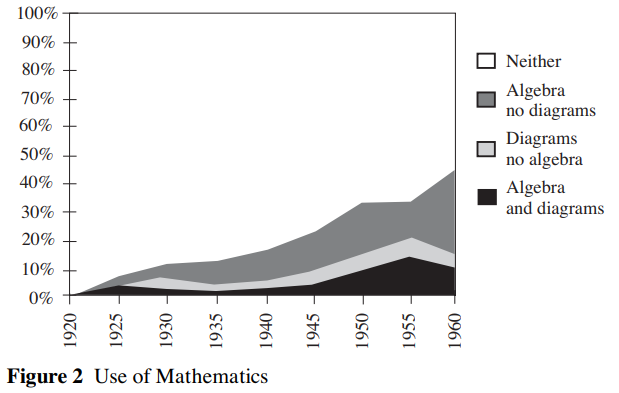
\includegraphics[width=0.75\textwidth]{4º Período/História do Pensamento Econômico/Tradução HPE/Tradução Tópico 7.2/figure 2.png}
    \end{figure}

O Uso da Matemática

Um aspecto importante desse processo foi o aumento do uso da matemática na economia, como mostrado na figura 2. Embora a matemática seja, em princípio, difícil de definir, as categorias usadas aqui eram inequívocas. O número de artigos que usavam algum tipo de matemática aumentou de zero em 1920 para 40 por cento em 1960. No entanto, a figura 2 subestima o aumento do uso da matemática em um sentido importante, pois o principal uso da matemática durante esse período está no desenvolvimento de argumentos teóricos. A matemática, além da análise estatística, raramente é usada no trabalho empírico. Como mostra a figura 3, a proporção de artigos teóricos que usavam álgebra aumentou muito mais rapidamente, atingindo quase 80 por cento em 1960. A figura 3 também confirma a visão comumente aceita de que, nas décadas de 1920 e início dos anos 1930, a AER era notavelmente menos matemática do que a QJE ou a JPE. Enquanto a matemática se estabeleceu na QJE e na JPE na década de 1920, não foi até a década de 1930 que isso aconteceu com a AER. No entanto, houve uma clara convergência em meados da década de 1950, quando uma proporção muito semelhante de artigos teóricos em todas as três revistas usava álgebra.

 \begin{figure}[H]
    \centering
    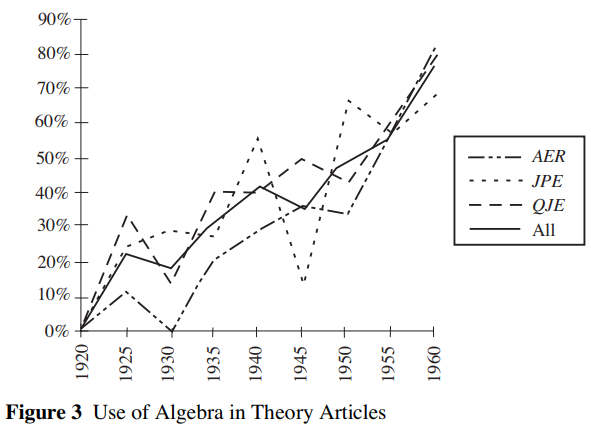
\includegraphics[width=0.75\textwidth]{4º Período/História do Pensamento Econômico/Tradução HPE/Tradução Tópico 7.2/figure 3.png}
    \end{figure}

Técnicas Empíricas

A econometria é comumente vista como tendo início nas décadas de 1920 e 1930 com o trabalho de Henry Schultz e Holbrook Working. A pesquisa revela, no entanto, que esses indivíduos contribuíram com uma grande proporção do trabalho de 1920 a 1960 que poderia ser classificado como econometria. A Tabela 1 mostra o número total de artigos usando análise de regressão (definida como envolvendo estatísticas diagnósticas) ou estatísticas descritivas que foram além de somas, médias, diferenças e similares (por exemplo, desvios padrão, análise de variância). Os números são realmente muito baixos.

Um indicativo de que essa amostra pode subestimar a aparência da econometria, como o termo é agora entendido, é fornecido na figura 4, que mostra a proporção de artigos empíricos na AER que usaram análise de regressão. Os anos na amostra de todas as revistas acontecem de ser anos em que a AEA publicou um número incomumente pequeno de artigos usando análise de regressão. No entanto, a Figura 4 confirma a imagem geral de que a análise de regressão começou a se estabelecer como uma ferramenta para pesquisa empírica na década de 1950. Muito mais comum era o uso de tabelas de estatísticas ou gráficos. A proporção de artigos que usaram gráficos ou tabelas aumentou de cerca de 50 por cento na década de 1920 para mais de 60 por cento em 1955-60.

\begin{figure}[H]
    \centering
    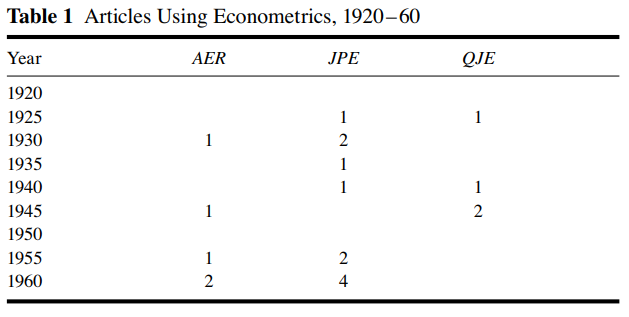
\includegraphics[width=0.75\textwidth]{4º Período/História do Pensamento Econômico/Tradução HPE/Tradução Tópico 7.2/table 1.png}
    \end{figure}

\begin{figure}[H]
    \centering
    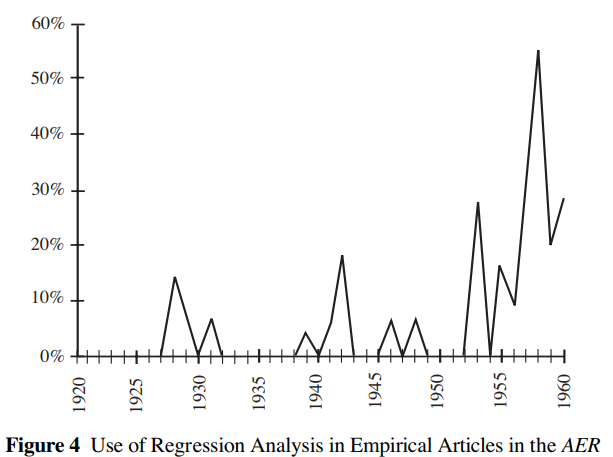
\includegraphics[width=0.75\textwidth]{4º Período/História do Pensamento Econômico/Tradução HPE/Tradução Tópico 7.2/figure 4.png}
    \end{figure}

\begin{figure}[H]
    \centering
    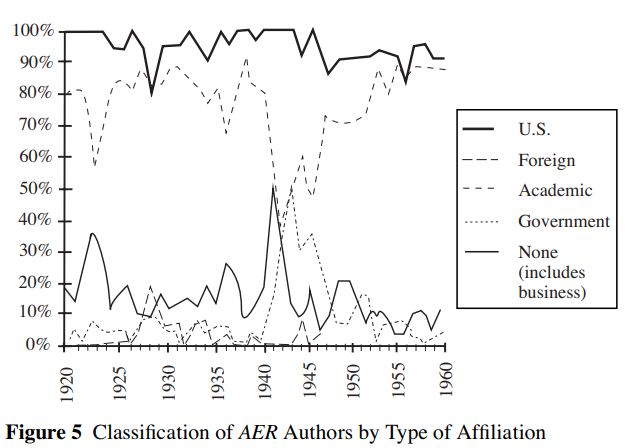
\includegraphics[width=0.75\textwidth]{4º Período/História do Pensamento Econômico/Tradução HPE/Tradução Tópico 7.2/figure 5.png}
    \end{figure}

\subsubsection{\textbf{Autores de Artigos de Revistas}}
Nacionalidade e Afiliação

As informações sobre os autores dos artigos do estudo são limitadas, mas ainda assim reveladoras. A Figura 5 classifica os autores da AER por tipo de afiliação. As afiliações dadas na revista são classificadas por país e por tipo de instituição. As categorias mais importantes são acadêmicas (universidades e institutos de pesquisa) e governamentais. A categoria rotulada como "nenhuma" inclui artigos para os quais nenhuma afiliação foi dada e um número muito pequeno que deu o nome de um negócio. A figura mostra que os artigos na AER foram esmagadoramente escritos por economistas baseados em instituições acadêmicas nos Estados Unidos. O contraste com as duas principais revistas britânicas examinadas em Backhouse 1997, que continham números significativos de artigos de economistas baseados fora da Grã-Bretanha, é marcante. Houve um breve aumento no número de contribuidores estrangeiros para a AER no final da década de 1920 e outro aumento para cerca de 10 por cento no final da década de 1940 e 1950. Igualmente significativa é a tendência de declínio no número de contribuidores para os quais nenhuma afiliação foi fornecida (a maioria dos quais eram presumivelmente não acadêmicos ou aposentados).

O principal evento subjacente à figura 5 é claramente a Segunda Guerra Mundial. Um grande número de economistas acadêmicos entrou para o serviço governamental durante a década de 1940, e depois retornou à academia após o fim da guerra. Embora houvesse exceções, como um artigo em 1943 sobre a curva de demanda de oligopólio vincada por Clarence Efroymson no Conselho de Produção de Guerra, praticamente todos os artigos eram sobre tópicos aplicados relevantes para a instituição onde o economista trabalhava. Assim, economistas do Office of Price Administration escreveram sobre controles de preços e a lacuna inflacionária, e economistas do Tesouro, do Bureau of the Budget e do Federal Reserve System escreveram sobre tributação, dívida governamental e política monetária. Uma das contribuições teóricas foi "‘Burden of the Debt’ and the National Income" (1944), de Evesey Domar, publicado enquanto Domar estava no Federal Reserve System. Em 1944-45, alguns artigos tentaram prever a renda nacional do pós-guerra.

Embora praticamente todos os contribuidores fossem baseados em instituições dos EUA, uma grande proporção nasceu no exterior. A Figura 6 classifica os autores da AER não por país de afiliação, mas por país de nascimento. Esta figura mostra um padrão notavelmente claro. Uma onda de imigração na década de 1920 foi revertida no início da década de 1930, seguida por um declínio dramático na proporção de contribuidores nascidos nos EUA para cerca de 50 por cento no final da década de 1940. Na década de 1950, a proporção se estabilizou em cerca de 70 por cento. Isso apoia a visão convencional de que a década de 1920 viu um influxo de emigrantes da Rússia e da Europa Oriental, e a década de 1930 viu migração em resposta à ascensão de Adolf Hitler na Alemanha. Embora esse influxo seja bem conhecido, a figura 6 mostra que ele tem um impacto muito significativo no fluxo de artigos sendo publicados que não se limitava a um pequeno número de indivíduos proeminentes, mas se estendia muito mais amplamente.

\begin{figure}[H]
    \centering
    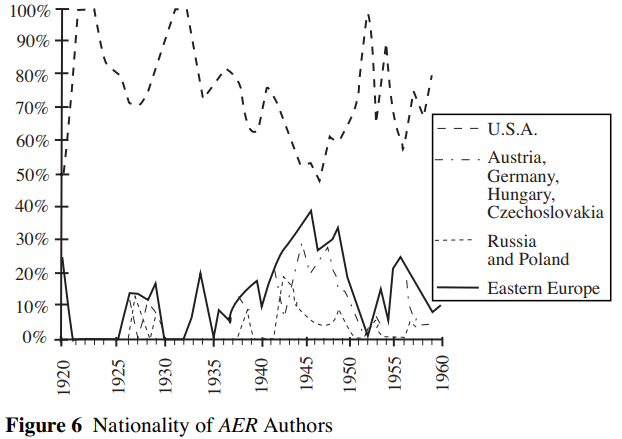
\includegraphics[width=0.75\textwidth]{4º Período/História do Pensamento Econômico/Tradução HPE/Tradução Tópico 7.2/figure 6.png}
    \end{figure}

Idade

Foi argumentado, notavelmente por Samuelson, que a transformação da economia que ocorreu nas décadas de 1930 e 1940 envolveu uma mudança geracional. Os jovens adotaram a economia matemática e a economia keynesiana de uma maneira que os economistas mais velhos não fizeram. Se isso estiver correto, deveríamos encontrar uma mudança na distribuição de idade dos colaboradores dessas revistas, especialmente entre os autores de artigos que usam matemática e artigos sobre macroeconomia. A Figura 7 mostra as idades médias dos colaboradores, e a Figura 8 mostra a distribuição de idades na amostra de cinco anos. A idade média era de cerca de 40 anos, aumentando ligeiramente ao longo do período. No entanto, houve variações notáveis na distribuição de idade. Não houve tendência na proporção de economistas com menos de 40 anos, mas a partir de 1945 em diante, houve uma queda na proporção de economistas com menos de 35 anos e, ainda mais dramaticamente, aqueles com menos de 30 anos contribuindo para essas revistas. Poderia ser argumentado que isso reflete a crescente profissionalização da disciplina e as crescentes demandas técnicas do assunto. Essas revistas estavam começando a ser consideradas prestigiosas, e os artigos nelas cada vez mais usavam matemática, o que dava uma vantagem aos economistas em seus trinta e poucos anos. Certamente não havia evidências de um influxo de jovens economistas nessas revistas na década de 1930.

\begin{figure}[H]
    \centering
    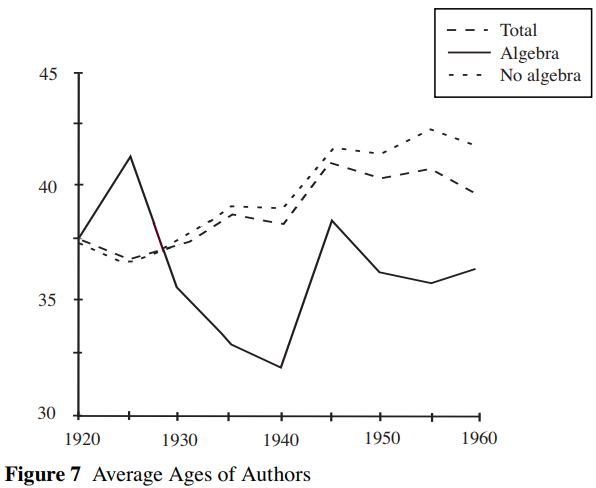
\includegraphics[width=0.75\textwidth]{4º Período/História do Pensamento Econômico/Tradução HPE/Tradução Tópico 7.2/figure 7.png}
    \end{figure}

\begin{figure}[H]
    \centering
    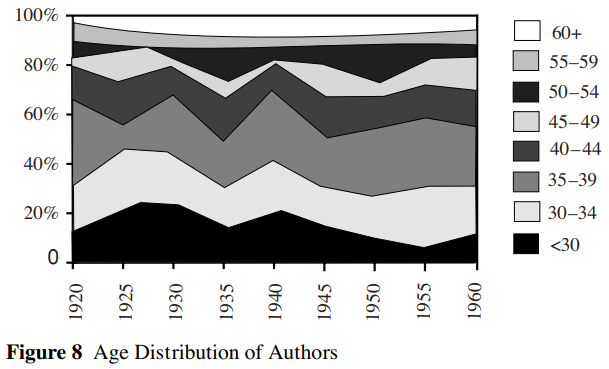
\includegraphics[width=0.75\textwidth]{4º Período/História do Pensamento Econômico/Tradução HPE/Tradução Tópico 7.2/figure 8.png}
    \end{figure}

De muito mais interesse é o padrão de idade dos autores de artigos que usam álgebra. Não há evidências de que os economistas matemáticos na década de 1920 e na primeira metade da década de 1930 eram mais jovens do que a média (embora deva ser lembrado que a amostra é pequena), mas durante meados a final da década de 1930 surgiu uma grande lacuna: em 1940 - 44 os economistas matemáticos tinham em média trinta e dois anos, sete anos mais jovens do que os autores de artigos que não usavam álgebra. Durante o final da década de 1940, essa lacuna fechou acentuadamente, com a idade média dos economistas matemáticos subindo para trinta e oito. A partir de 1950, a lacuna se estabilizou em cerca de cinco anos. Isso é consistente com a teoria de que a economia matemática foi introduzida por uma nova geração que entrou na profissão no final da década de 1930. O aumento na idade dos economistas matemáticos no final da década de 1940 apoia essa teoria, pois nesse período os entrantes na profissão normalmente teriam sido mais velhos, tendo passado vários anos nas forças armadas. O aumento na idade média dos usuários de álgebra na década de 1950 em comparação com a idade média no final da década de 1930 e início da década de 1940 pode ser explicado pelas crescentes demandas técnicas do assunto e pelo fato de que essas técnicas estavam se tornando muito mais amplamente aceitas.

\subsubsection{\textbf{Instituições}}
A análise das afiliações institucionais dos autores pode lançar luz sobre dois fenômenos: o domínio de um pequeno número de instituições e as mudanças nas instituições líderes à medida que o assunto foi transformado. Na medida em que as instituições estão associadas a abordagens particulares da economia (Wisconsin com institucionalismo, o Instituto de Tecnologia de Massachusetts [MIT] com economia neoclássica), isso pode nos ajudar a documentar a transformação do assunto. No entanto, muitas instituições não podem ser associadas a escolas de pensamento específicas. De 1925/26 a 1950/51, os principais produtores de Ph.D. em economia foram Harvard (600), Columbia (394), Wisconsin (282), Cornell (244), Chicago (243) e Illinois (218) (Bowen 1953, citado em Moggridge 1995). Desses, Columbia tinha uma forte presença institucionalista (Clark e Mitchell), mas Harold Hotelling também estava lá fazendo economia matemática, embora Arrow (1990, 46) afirme que até 1940, quando era estudante, a ênfase do Departamento de Economia "era quase inteiramente em análises empíricas e institucionais". Thorstein Veblen estava em Chicago no início do período, e Knight estava lá no final. Harvard também não pode ser facilmente associada a uma única escola: Taussig, Chamberlin e Schumpeter claramente não eram institucionalistas, mas também não eram neoclássicos. Além de Samuelson, Harvard produziu John Kenneth Galbraith.

As instituições podem ser analisadas considerando-se as instituições nas quais os autores estavam baseados quando seus artigos foram publicados ou vinculando os autores às instituições das quais se formaram, definidas aqui como a instituição da qual um Ph.D. foi obtido. Os dados são mostrados nas tabelas 2 e 3. A amostra da AER foi escolhida para evitar o viés em direção a Chicago e Harvard que resultaria do uso do JPE e do QJE.

A Tabela 2 mostra pouca mudança no grau de concentração de afiliação. Em todas as décadas, exceto a década de 1940, as três principais instituições representavam cerca de 15 por cento dos artigos, as dez primeiras por volta de 38 por cento, e as quinze primeiras por volta de 45 por cento. A década de 1940 viu uma redução na concentração, talvez porque um número desproporcional de economistas publicadores de instituições líderes foram atraídos para o trabalho de guerra. Seja qual for a razão, as proporções de concentração do pré-guerra foram restabelecidas na década de 1950.

A história em relação às instituições de Ph.D. é mais mista, embora o que se destaca é o grau muito maior de concentração. As três principais instituições de Ph.D. representaram quase 50 por cento dos artigos, as dez primeiras por volta de 75 por cento, e as quinze primeiras por mais de 80 por cento. Se a formação de Ph.D. é importante para determinar a direção do assunto, é necessário considerar apenas um número muito pequeno de instituições.

Embora o sistema fosse altamente concentrado, houve mudanças notáveis nas instituições dominantes, como mostrado em ambas as tabelas. Nas três primeiras décadas do período, economistas baseados em Princeton, Columbia e Harvard dominaram a AER, enquanto na década de 1950 as instituições líderes eram Berkeley, MIT e Stanford. Também é digno de nota o aumento constante de Chicago para o quarto lugar na década de 1950. Tendo em vista o declínio do institucionalismo, muitas vezes datado da década de 1930, é significativo que Wisconsin tenha caído de cerca de sétimo lugar na década de 1920 para o décimo primeiro na década de 1950. No entanto, o declínio na participação de artigos da AER por Ph.D.s de Wisconsin é ainda mais acentuado, de 12 por cento na década de 1920 e 10 por cento na década de 1930 para apenas 5 por cento na década de 1950. Nas décadas de 1940 e 1950, a AER foi dominada por economistas treinados em Harvard, que escreveram tantos artigos quanto economistas das duas próximas instituições, Columbia e Chicago, combinados. Na década de 1920 e 1930, Ph.D.s de Harvard e Columbia publicaram artigos da AER em números iguais na década de 1950.

\begin{figure}[H]
    \centering
    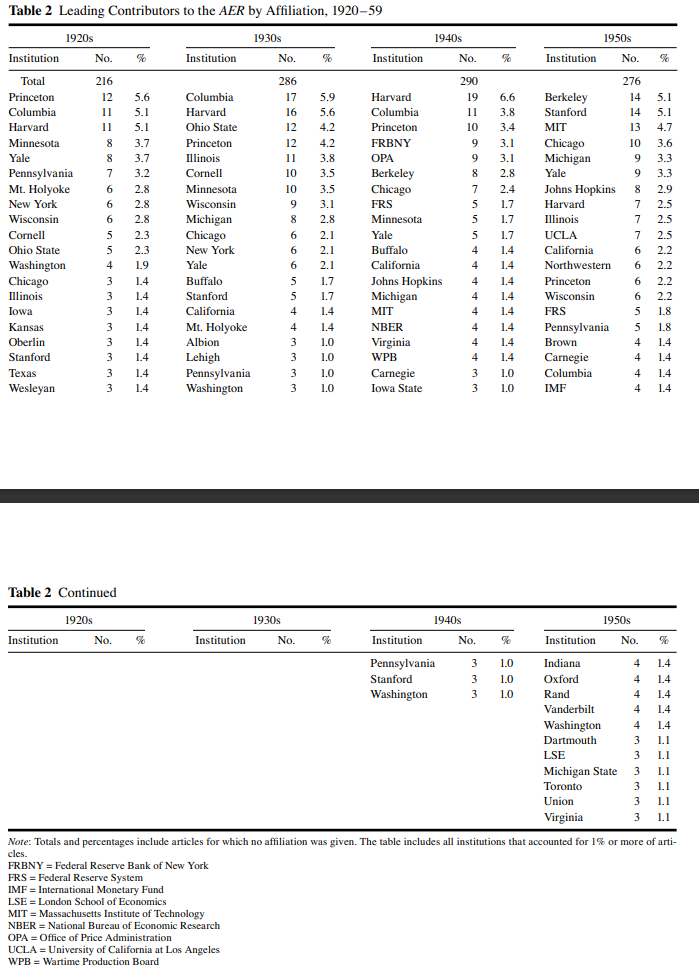
\includegraphics[width=0.75\textwidth]{4º Período/História do Pensamento Econômico/Tradução HPE/Tradução Tópico 7.2/table 2.png}
    \end{figure}

\begin{figure}[H]
    \centering
    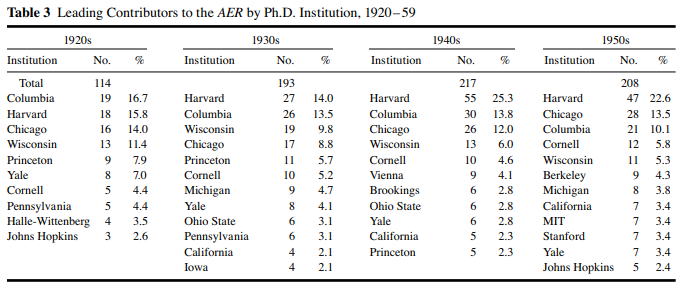
\includegraphics[width=0.75\textwidth]{4º Período/História do Pensamento Econômico/Tradução HPE/Tradução Tópico 7.2/table 3.png}
    \end{figure}

\subsubsection{\textbf{Conclusão}}
A análise da economia dos EUA confirma muitas das histórias que contamos sobre a transformação da economia entre 1920 e 1960. Imigrantes da Europa tiveram um impacto quantitativo significativo, indo além da influência de um pequeno número de indivíduos proeminentes. As evidências apoiam a ideia de que a década de 1930 foi um período crucial na matematização do assunto, associada ao influxo de uma geração mais jovem de economistas. A econometria, como o termo é agora entendido, no entanto, não decolou até a década de 1950. Embora as evidências estejam longe de ser conclusivas, é possível ver padrões que são consistentes com o declínio do institucionalismo começando na década de 1930: a participação decrescente de artigos da AER produzidos de Wisconsin e por Ph.D.s de Wisconsin; o surgimento repentino de Stanford, MIT e Berkeley na década de 1950; e possivelmente o deslocamento de Columbia por Harvard. Isso é o que a maioria das pessoas esperaria.

A análise também sugere algumas características da transformação da economia dos EUA que de outra forma poderiam ter sido esquecidas. O impacto massivo da guerra na profissão é o mais óbvio. Em um momento crucial, um grande número de economistas deixou a academia para trabalhar no governo ou no exército. Igualmente importante, a matematização do assunto, embora tenha avançado muito, estava longe de estar completa em 1960. Se a ortodoxia dominante é vista como envolvendo o uso de modelos de otimização formal que são testados usando técnicas econométricas, o assunto ainda tinha um longo caminho a percorrer. Por exemplo, até 1960, 71 por cento dos artigos empíricos não usavam análise de regressão. O aumento dramático de 1955 a 1960 na proporção de artigos que usavam álgebra, mas nenhum diagrama, sugere que uma mudança substancial estava ocorrendo justamente quando o período terminava. Esta é uma característica da transformação da economia dos EUA que as contas de figuras-chave, como Arrow, Samuelson ou Friedman, podem facilmente ignorar.

No entanto, uma das conclusões mais significativas surge não da análise estatística, mas da classificação dos artigos. O fato de que era difícil classificar muitos artigos da primeira metade do período como teóricos ou empíricos, mas menos difícil em direção ao final do período, é uma evidência de que uma mudança significativa ocorreu na economia dos EUA durante esse período. Embora a mudança tenha sido indubitavelmente associada à transformação da economia dos EUA do pluralismo pré-guerra para o neoclassicismo pós-guerra - pois a divisão entre teórica e empírica é uma característica do tipo de economia que tem cada vez mais dominado o assunto no período pós-guerra - ela não é sinônima com isso. A economia acadêmica estava se expandindo, juntamente com todo o sistema de educação superior, e o assunto estava cada vez mais capaz de apoiar uma variedade de revistas, como as discutidas aqui, lidando com questões que eram de preocupação principalmente apenas para economistas acadêmicos. A economia estava se tornando, juntamente com muitas outras disciplinas, mais voltada para dentro. Ambas as técnicas teóricas e empíricas se tornaram mais formais, permitindo que fossem distinguidas uma da outra de uma maneira que não era possível na década de 1920.


\section{\textbf{(OPCIONAL) : Claveau e Gingras (2016)}}
\subsection{\textbf{Macrodinâmica da Economia: Uma História Bibliométrica}}
As disciplinas acadêmicas cresceram enormemente desde a Segunda Guerra Mundial e a economia não é exceção. Entre os artigos de economia indexados na Web of Science da Thomson Reuter, cerca de mil foram publicados em 1956, enquanto quase vinte mil são publicados anualmente hoje. Esse aumento equivale a uma taxa de crescimento anual média entre 5 e 6 por cento, que é comparável ao crescimento anual global da ciência no mesmo período (Larsen e von Ins 2010). Para ter certeza, esses números dão apenas uma indicação aproximada do crescimento da economia, porque a Web of Science não indexa todos os artigos acadêmicos, mas apenas um subconjunto que aparece nas principais revistas acadêmicas ao redor do mundo. No entanto, esses números aproximados são suficientes para indicar a magnitude das transformações que afetaram a escala da pesquisa científica em geral e em economia em particular ao longo do último meio século.

Embora os tipos tradicionais de análise do desenvolvimento da economia - análise textual de documentos e arquivos publicados, entrevistas, reconstrução biográfica de figuras importantes, genealogia de conceitos e métodos - permaneçam úteis, ferramentas específicas valem a pena explorar para entender a estrutura global e morfologia da economia à medida que mudou ao longo da segunda metade do século XX. Este artigo introduz uma combinação dessas ferramentas para a história da economia. Combinamos bibliometria com análise de rede dinâmica para identificar uma estrutura de especialidade em mudança na economia desde o final dos anos 1950 até 2014. Mapeamos como as especialidades surgiram, cresceram em relação umas às outras e (para algumas delas) desapareceram. Nossos resultados se combinam bem com relatos mais narrativos da história recente da economia (por exemplo, Backhouse 2002, cap. 14; Backhouse e Cherrier 2014; e Morgan e Qin 2015): eles confirmam certas afirmações que podem ser encontradas na literatura existente e identificam padrões intrigantes que convidam a uma pesquisa qualitativa mais aprofundada (veja a seção 5)

Dados bibliométricos têm sido usados na economia, mas essencialmente para estatísticas descritivas com fins avaliativos - por exemplo, classificações de revistas e autores mais citados (Kalaitzidakis, Mamuneas e Stengos 2003; Kodrzycki e Yu 2006; Ritzberger 2008; Stern 2013; Zimmermann 2013; Card e DellaVigna 2013). Apenas alguns artigos que usam dados bibliométricos da economia não têm um objetivo avaliativo explícito, concentrando-se mais na estrutura da autoria e nos métodos usados em artigos em um pequeno número de chamadas revistas de topo (Hamermesh 2013), na identificação das características dos artigos mais citados (Kim, Morse e Zingales 2006), ou na descrição da evolução do número de artigos em um determinado domínio de pesquisa (por exemplo, Silva e Teixeira 2008; Silva e Teixeira 2009).

Até onde sabemos, este artigo é o primeiro no campo da história da economia a combinar dados bibliométricos e análise de rede dinâmica. Além disso, nosso corpus de cerca de 415.000 documentos é muito maior do que os corpora usados na maioria dos outros estudos sobre a história da economia. O artigo segue os passos de vários estudos que mostraram que a bibliometria e a análise de rede são particularmente adequadas para estudos de grande escala do desenvolvimento histórico de disciplinas científicas e especialidades (Garfield 2009; Cole, Cole e Dietrich 1978; Boyack, Börner e Klavans 2009; Gingras 2010a, 2010b, 2010c; Gingras e Schinckus 2012). A grande vantagem de combinar bibliometria e análise de rede é a possibilidade de detectar e visualizar algoritmicamente padrões na produção de pesquisa de grandes grupos. Padrões que podem permanecer ocultos ou embaçados com métodos históricos padrão de repente vêm à luz.

\subsubsection{\textbf{1. Estrutura Conceitual: Economia como uma Rede de Especialidades}}

Em qualquer disciplina científica madura, a comunidade científica é de fato composta de subunidades relativamente autônomas (as especialidades) nas quais o novo conhecimento é tornado público por meio de publicações. Essas diferentes especialidades, que surgiram ao longo do tempo com o crescimento morfológico e a subsequente divisão do trabalho dentro da disciplina, estão mais ou menos conectadas entre si, assim como a própria disciplina está mais ou menos conectada a outras disciplinas que compõem o campo científico global. Enquanto a disciplina geralmente corresponde ao treinamento básico de nível de entrada (BA) em um departamento universitário, a especialidade corresponde mais ao nível de pesquisa aprendido nos níveis de mestrado e doutorado e leva à produção de novos conhecimentos (Hagstrom 1965; Cole e Cole 1973; Whitley 1976; Whitley 2000; Bourdieu 2004; Wray 2005).

\end{document}